\section{Opportunities and risks of autonomous vehicle}


\subsection{Autonomous Vehicle: Opportunity for urban mobility}
"Urban mobility is a dynamic system that has had a (slow) natural evolution" \cite{medina-tapia_exploring_2018}. With the development of technology, manuals vehicles will be replaced by AVs and vehicles will have the capable communicate and cooperate with each other. The society will expect significant innovations in mobility services. Moreover, the way people move around the urban environment is primed for profound changes , and cities will progressively become Smart Cities which will permit the vehicles to interact with the urban infrastructure.
The main goals of AV are to create a safer, more reliable, more efficient, more comfortable and more affordable way of travel. It is also expected to reduce traffic congestion, gas emission, fuel consumption, etc. When the autonomous system is activated, "the driver is replaced by a computer system to improve specific dimensions of driving such as safety, traffic fluidity, ecology, and economy".\cite{chehri_autonomous_2019} \smallskip

\begin{center}
    \begin{figure}[ht!]
        \centering
        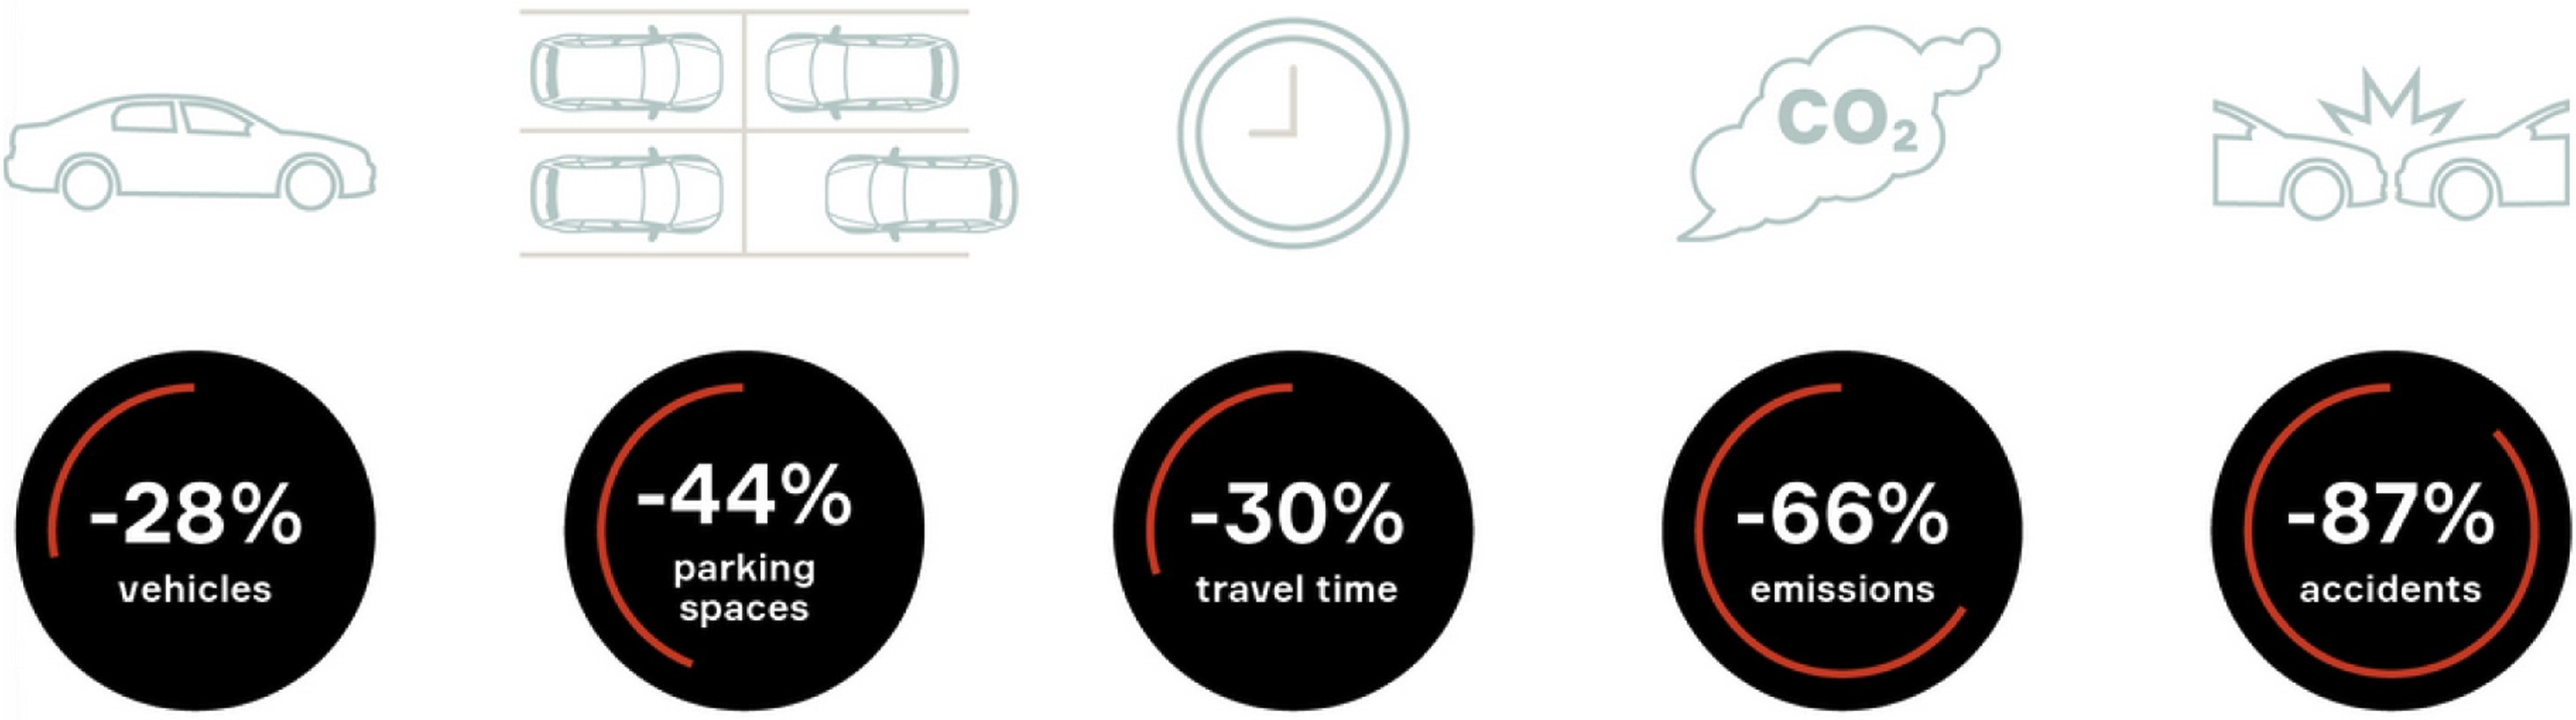
\includegraphics[width=400px, keepaspectratio]{imports/benefi_of_AVs..jpg}
        \caption{The benefit of autonomous vehicle in sustainable cities.}  \cite{chehri_autonomous_2019}
    \end{figure}
\end{center}

First of all, the automatization of the driving process (AVs) could reduce the generalized travel cost and the traffic congestion. Simulation studies show that AVs are capable of reducing collision on the road by eliminating or minimizing human errors and improving flow management, it could also make the real time-navigation more efficient. As a consequence, the AVs will allow increasing the urban road capacity due to platoon formations in urban roads and will reduce the amount of vehicle by 30\% in crowded city. Furthermore, they will increase the efficiency of infrastructure through better vehicle control. \smallskip

Secondly, the operation of transit and mobility services can be improved. The shared routes for theses services will be more accessible, reliable, and flexible. The AVs can make the mobility services more affordable and the transit operation by public services less subsidized. So that the transport services are increasingly capable of improving safety, reliability, security, and productivity. It could also benefit the citizen by offering an alternative mode of transportation and perhaps more efficient.\smallskip

Thirdly, the autonomous technologies can reduce greenhouse emissions by two third, thus reducing the pollution. The AVs make vehicles and infrastructure more environmentally friendly. It also encourages the transition from personal ownership to carpooling services. The ownership of the vehicle will be less necessary or unnecessary for users. Therefore, the number of vehicles will be reduced. The Avs could eliminate the waves of traffic created by stop-and-go behavior (where humans, rather than road accidents, create changes in speeds). This in turn will not only save people time, but decrease the time their cars are on the roads and therefore reduce emissions. \smallskip

Fourthly,  the AVs improve road safety. Beside of reducing traffic accidents by eliminating or minimizing human errors, it can make the journey less stressful and more comfortable. The United States Department of Transportation (USDOT) predicts that autonomous technologies has the potential to reduce traffic accidents by 87\%. \smallskip

Furthermore, the AVs have some other contribution to user, sustainable and cities and society. They benefit minors, the elderly, disabled, tired, drunk, or inattentive people by providing a greater freedom of mobility. Many seniors and people with disabilities cannot currently drive, even with vehicle modifications that help others drive safely. AVs could provide many more users access to the open road and to independence. It improves care and services dedicated to reduced mobility people. In addition, AVs can increase the life span of the vehicle by reducing the travel time . As a result, the maintenance cost can be reduced greatly.



\subsection{Challenges autonomous vehicles need to be overcome }

\subsubsection{Difficulty of understanding human gesture}

In the paper \cite{brooks_robotic_2017} the author discussed the difficulty for an autonomous car to understand human gesture. Figuring out of the way people pause and move is one of the problems yet to be solved even though some pedestrian detection mechanism have been mentioned in the previous part. An AV cannot tell what any human driver could decide instantaneously. For instance, the human driver can tell that people chatting on the street side have no intention to cross the road. On the other hand, if one suddenly turns away from the other in the direction of the street, it means that he or she is about to cross.
In the above situation, AVs lack the ability to assess the road safeness to move on. Should the AV decide, for safety reasons, to let the person start crossing the road by slowing down the vehicle or eventually coming to a halt in order to avoid hitting the person. Undoubtedly, this will slow down the traffic. If the person’s intention is guessed wrongly, the course of action will annoy the human driver that is stuck behind the autonomous cars. AVs would then create inconvenience.


\subsubsection{Anti-social act}

The flip side of AVs is giving the owners the opportunity to be anti-social. People will be tempted to take advantage of the road with their AVs without consideration for others. For instance, people will hop out of their cars in front of the shop to get something while leaving the car at an illegal parking spot, knowing well that AVs will take care of themselves and get out of the way if someone’s way is blocked. As a result, the traffic will be slowed down by this selfish act of the car owner and increase greenhouse gases emissions. Unattended cars will be everywhere.

\subsection{Implementation of security measure on an autonomous vehicle}

\subsubsection{Multi-layer IDS for autonomous vehicle}

A paper \cite{straub_cybersecurity_2017} described several component systems which comprised of an AV intrusion detection system (IDS) to detect suspicious activities, ranging from conventional local attacks to complicated manipulation attacks which are designed to manipulate the actions taken by the car. The multi-layer IDS proposed consists of four layers:
\begin{itemize}
  \item Vehicle-level intrusion detection. This IDS performs analysis on information without accessing to the larger network so it could be used to evaluate the trustworthiness of the network resources. However, this level is limited to the attacks that it can detect and the symptoms that it consider malicious as it does not try to compare data. Analysis performed are based on the data collected by the car to identify trends and patterns. The concept of mutually verifiable information implies that the user’s car can verify the information sent by the other car using their own sensor.

  \item Vehicle area network intrusion detection. This IDS scans the data transmitted between vehicles in real time with Vehicular Ad-Hoc Network(VANET) to look for anomalies and signs of malicious activity.
  
  \item Wide area vehicle coordination and traffic management. The third level securing information beyond the local VANET, using the roadside units (RSUs) for collection and transmission of data.
  
  \item Multiple areas or multiple layers of self-driving vehicle manipulation detection. 
\end{itemize}

\subsubsection {Reputation rating }
The reputation rating defines the trustworthiness of a car, the higher the reputation, the more likely the data emitted by the car will be taken into consideration of the analysis and calculation. If the rating drops below a certain level, it will be considered suspicious. Falling below limit, it will be categorized as malicious. The node with the highest rating serves as the gateway nodes to other proximate VANETs.

\subsubsection{Implementation difficulties}
This proposed IDS relies greatly upon the presence of RSUs but the feasibility of implementing RSUs cannot be adequately predicted at this time. Besides, the effectiveness of IDS will depend on the level of collaboration and coordination between vehicle manufacturers and their level of sharing of knowledge. 

Moreover, the authority who controls the cybersecurity responsibility (beyond the car level) will undoubtedly impact the priority of the cybersecurity system, the way it operates, and the configuration.